\subsection*{j. La información del cliente que más órdenes haya efectuado. Mostrar el número de órdenes que ha realizado.}

Primero agrupamos la tabla \textit{orders} por \textit{customerid} para contar el total de órdenes efectuadas usando la función COUNT sobre \textit{orderid}. Nombramos este agregado como \textit{numorders} y llamaremos a esta operación $T$. Después, buscamos el valor máximo de órdenes registradas aplicando la función de agregación MAX sobre \textit{numorders} en una nueva agrupación. Este paso se guarda como $T_{max}$. Hacemos un join de $T$ y $T_{max}$ indicando en la condición $\theta$ que \textit{numorders} debe ser igual a \textit{MaxOrders}, filtrando así únicamente el o los IDs de cliente con la máxima participación. Por último, aplicamos un join natural con la tabla \textit{customer} para obtener toda la información del cliente ganador, y usamos una proyección para presentar todos sus atributos junto con la columna adicional \textit{numorders}.

Expresión:
\begin{equation}
\begin{split}
T &= \gamma_{customerid;\, \text{COUNT}(orderid) \rightarrow numorders}(orders) \\
T_{max} &= \gamma_{\text{MAX}(numorders) \rightarrow MaxOrders}(T) \\
\text{Resultado} &= \pi_{customer.*,\, numorders} (customer \bowtie (T \bowtie_{numorders = MaxOrders} T_{max}))
\end{split}
\end{equation}

Resultados obtenidos:

\begin{figure}[h!]
\centering
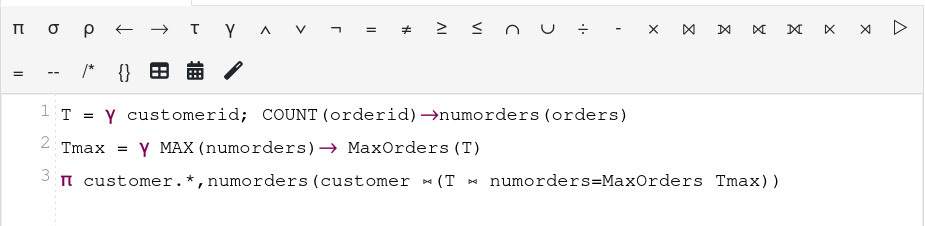
\includegraphics[width=0.8\textwidth]{imagenes/2j(1).png}
\caption{Consulta 2j.}
\end{figure}

\begin{figure}[h!]
\centering
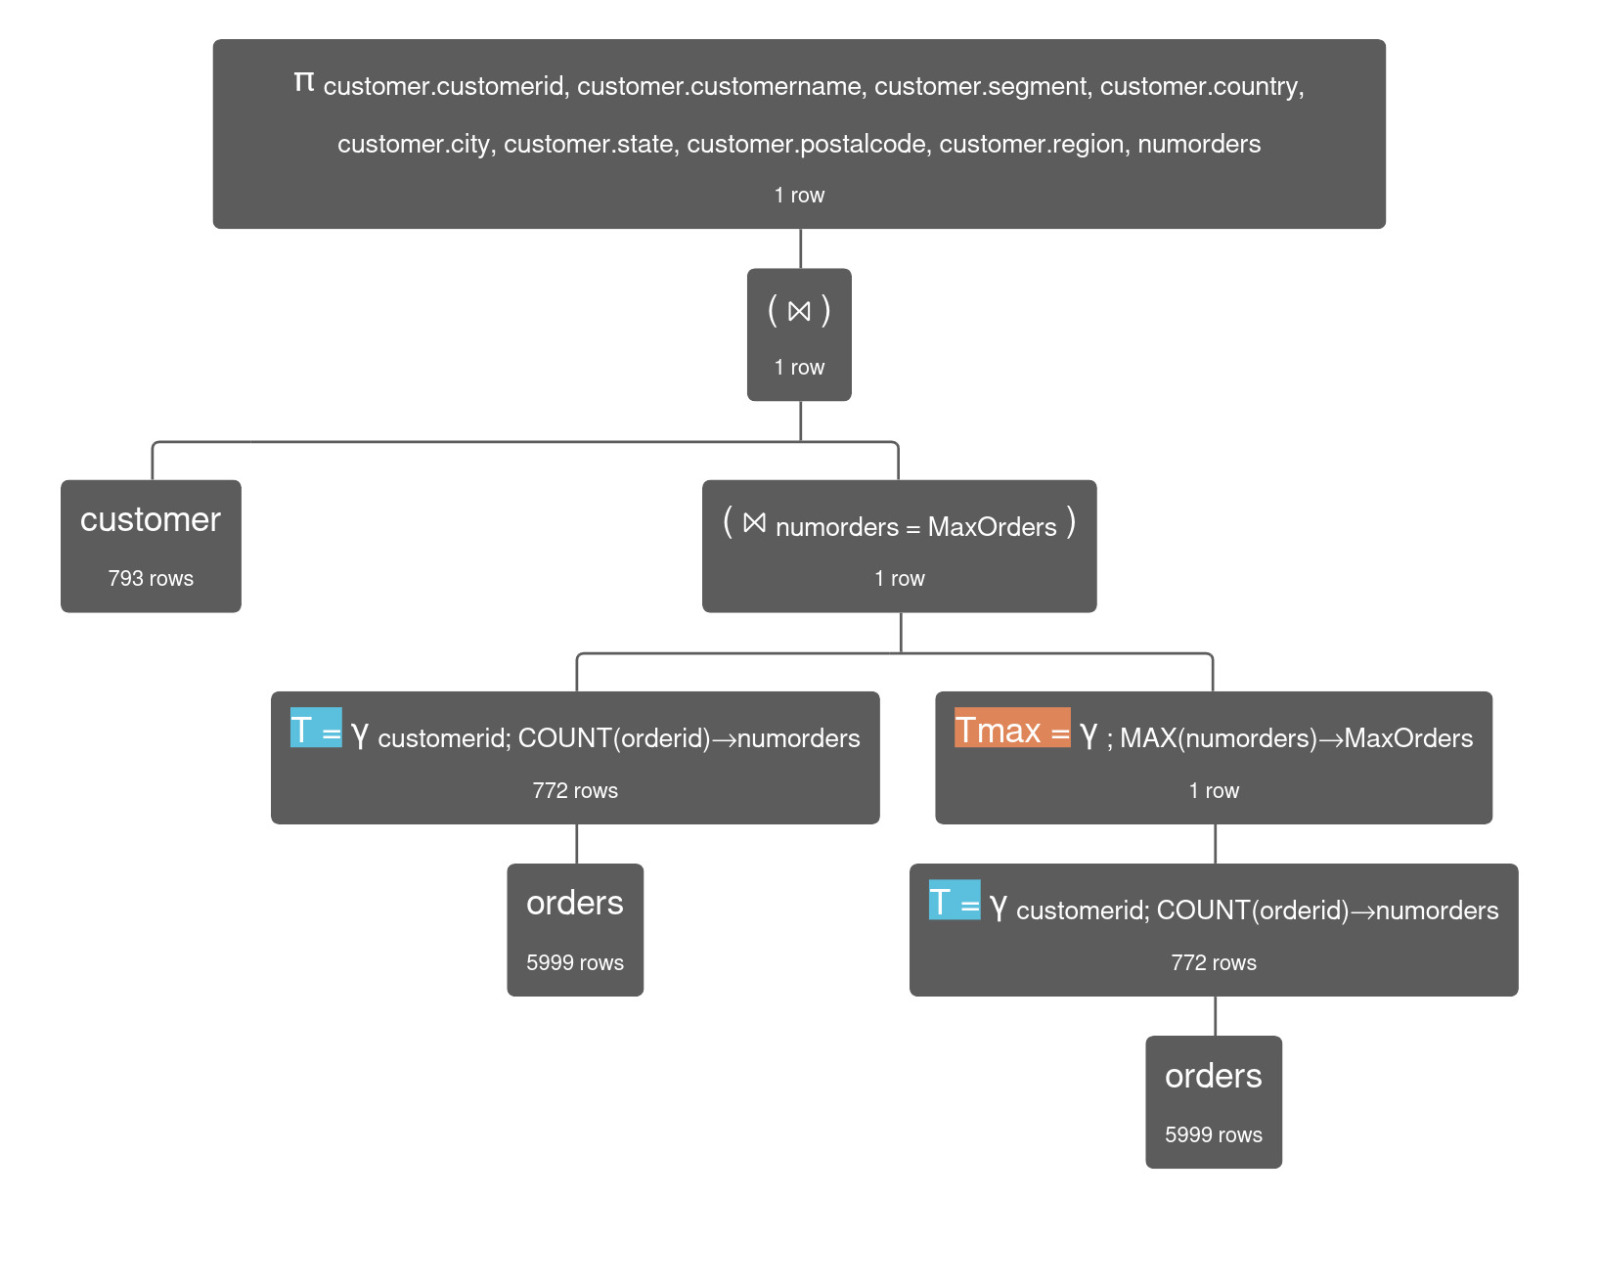
\includegraphics[width=0.8\textwidth]{imagenes/2j(2).png}
\caption{Árbol de consulta 2j.}
\end{figure}

\begin{figure}[h!]
\centering
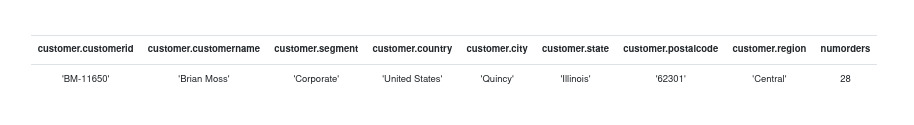
\includegraphics[width=0.8\textwidth]{imagenes/2j(3).png}
\caption{Resultado de consulta 2j.}
\end{figure}
